\subsection{Estimation of The Baseline Model} 
\label{sec:estimation_ble}

\subsubsection*{Sample Period and Prior Distributions}

In this section, we compare the empirical fit of the 3-equation New Keynesian model under  REE, BLE and SAC-learning. We augment the Taylor rule with an i.i.d monetary policy shock and an interest rate smoothing parameter to allow the model to match the inertia of the historical interest rate: 
\begin{equation}
r_t = \rho_r r_{t-1} + (1-\rho_r) (\phi_{\pi}\pi_t +\phi_x y_t) +\epsilon_{r,t}.
\label{eqn:3_1}
\end{equation}

\noindent

We estimate the small-scale system of  (\ref{nkmodel}) and (\ref{eqn:3_1}) for the U.S economy over the period 1966:I-2016:IV using quarterly macroeconomic data. We also investigate whether our results are sensitive to structural breaks such as the large volatility reduction for most macroeconomic time series during the mid-80s, often referred to as the Great Moderation, or the near-zero level of nominal interest rates that followed the 2007-08 crisis period. 
%The U.S economy has experienced a large volatility reduction in most macroeconomic parameters in mid-80s, often referred to as the Great Moderation. Nevertheless we consider the entire sample period in this section: Inflation is highly persistent over the entire sample period, while its persistence is substantially reduced if we consider the post Great Moderation period. The highly persistent series allow us to illustrate the persistence amplification under the BLE estimation. Furthermore, empirical studies involving the U.S interest rate typically do not cover the post-2007 period due to concerns over the zero lower bound. Therefore, while we ignore the potential impact of the ZLB constraint in our main estimations, we show that the results are robust to different sample periods later on\footnote{Furthermore, recent studies show that, if there are any biases at all on the estimated parameters related to ignoring the ZLB, these are limited to steady-state and monetary policy related parameters, while the rigidity and structural shock parameters remain unaffected. See \citet{hirose2016parameter} and \citet{hirose2016zero} for more details.}.
We use the following measurement equations for output gap, inflation and interest rate\footnote{See Appendix \ref{app_data} for more details on the observable variables.} without measurement errors:
\begin{equation}
\begin{cases}
log(y_t^{obs})= \bar{\gamma}+y_t \\
log(\pi_t^{obs})=\bar{\pi} + \pi_t\\
log(r_t^{obs}) = \bar{r} + r_t, \\
\end{cases}
\label{eqn:3_2}
\end{equation}
\noindent
where we use the cycle component of HP-filtered quarterly output as our measure of output gap\footnote{As shown in the next section, our main results are not sensitive to the choice of output gap measure.} ${y_t^{obs}}$, while $ \pi_t^{obs} $ and $r_t^{obs} $ denote the quarterly historical inflation and interest rate series respectively. $\bar{\gamma}, \bar{\pi} $ and $ \bar{r}$ correspond to the historical mean levels of output gap, inflation and interest rate. The model is estimated using the same prior distributions under all three specifications, which guarantees that any differences that arise between the estimations is due to the difference in the expectation formation rule. The prior distributions are kept close to those commonly assumed in the literature: the risk aversion coefficient $\tau= \frac{1}{\varphi}$ is assigned a gamma distribution centered at 2 with a standard deviation of 0.5, covering values of approximately up to four. The slope of the Phillips curve $ \gamma$ is assigned a Beta distribution with mean $ 0.3$ and standard deviation $0.15$  which falls somewhere between the prior in An \& Schorfheide (2007) and Smets \& Wouters (2007), covering both flat and steep cases for the Phillips curve\footnote{In particular if we denote the nominal price stickiness as $\omega$, its relation with $\gamma$ is given as $\gamma=\frac{(1-\lambda \omega)(1-\omega)}{\omega}$ (Gali, 2008). Smets \& Wouters (2007) assume a prior for $\omega$ with mean $0.5$.}.  The policy response parameters for output gap and inflation are assigned beta distributions centered around $ 0.5$ and $ 1.5$, which are standard values associated with the Taylor Rule in the literature. The autocorrelation coefficients have a Beta distribution centered at 0.5, and the standard deviations for the shock processes are assumed to follow an Inverted Gamma distribution with a mean of 0.1 and standard deviation of 2, same as in Smets \& Wouters (2007). The priors for the steady-state inflation rate, output growth and interest rate are normal distributions centered at their pre-sample means of $0.47$, $-0.2$ and $0.72$ respectively, where the pre-sample period covers data from 1954:I to 1965:IV.  Finally, we fix the HH discount rate $\lambda$ at 0.99, which is a standard assumption in most empirical studies.\\


%\begin{table}

%\centering
%\caption{\small Prior Distributions for the Structural Parameters of the Small-Scale NKPC Model.}
%\label{table:table2}
%\vspace{5 mm}
%\begin{tabular}{l|l|l|l}

%Parameter & Dist. & Mean & St. Dev   \\
%\hline
%\hline
%$\eta_y$ & Inv Gamma & 0.10 & 2   \\
%$\eta_{\pi}$ & Inv Gamma & 0.10 & 2  \\
%$\eta_r$ & Inv Gamma & 0.10 & 2   \\
%$\bar{\pi}$ & Normal & 0.47 & 0.25  \\
%$\bar{y}$ & Normal & -0.2 & 0.25  \\
%$\bar{r}$ & Normal & 0.72 & 0.25 \\
%$\frac{1}{\psi}$ & Gamma & 2 & 0.50  \\
%$\gamma$ & Beta & 0.3 & 0.15   \\
%$\rho_y$ & Beta & 0.50 & 0.20   \\
%$\rho_{\pi}$ & Beta & 0.50 & 0.20  \\
%$\rho_r$ & Beta & 0.50 & 0.20  \\
%$\phi_y$ & Gamma & 0.50 & 0.25  \\
%$\phi_{\pi}$ & Gamma & 1.5 & 0.25  \\


%\end{tabular}
%\label{table1}
%\end{table}

\subsubsection*{Convergence Diagnostics}
Table \ref{table3} presents the posterior estimation results for the BLE, RE and SAC-learning models.\footnote{BLE and REE models are estimated using the Dynare toolbox (Adjemian et. al, 2011), while our own toolbox is used for the SAC-learning estimations since it requires an additional learning step in the filter recursions. The posterior distributions are constructed using the Metropolis-Hastings algorithm with 250000 draws, using the first 50000 as the burn-in sample. The step size for the scale parameter of the jumping distribution's covariance matrix is adjusted in both models to obtain a rejection rate of ~70\% in both models, which is in the commonly assumed {appropriate} range for the MH algorithm.} Before moving onto the estimation results, we first briefly discuss the convergence diagnostics of {BLE} and SAC-learning. Under BLE, initializing both $\beta_y$ and $\beta_{\pi}$\footnote{In this section we switch to the notation $\beta_y$ and $\beta_{\pi}$ instead of $\beta_1$ and $\beta_2$ to make the exposition more clear.} at fairly low values of 0.5 and using a convergence criterion $\epsilon=10^{-5}$, our estimation algorithm takes only 5 steps to converge\footnote{The results are robust to initial values of $\beta_y$ and $\beta_{\pi}$.}. The resulting BLE is $\boldsymbol (\beta_y^{*},\beta_{\pi}^{*})=(0.88,0.89)$ at the final step. This is fairly close to the sample-autocorrelation moments of the data over this period, which is $(0.87,0.89)$. The left panel of Figure \ref{nkm_convergence} shows the norm distances between two consecutive sets of $\pmb{\beta}^{(k)}$ and $\theta^{(k)}$ at each step $k$, both of which rapidly converge towards 0. The largest eigenvalue of the Jacobian matrix $DG(\pmb{\beta}^{(k)},\theta^{(k)})$ remains strictly inside the unit circle during the estimation, and stabilizes after the second step. The right panel of the same figure shows the convergence of Algorithm I towards $\pmb{ \beta}^{*} $ at the estimated posterior mode with randomized initial values, suggesting that the estimated equilibrium is the unique iteratively E-stable BLE. Similar results emerge when we examine the Monte Carlo simulations of the model under SAC-learning in Figure  \ref{nkm_sac_MC}: the left panel shows the histograms of $\beta_y$ and $\beta_{\pi}$ over 1000 simulations under decreasing gain learning, while the right panel shows the constant gain equivalent with a small gain value of $0.001$. It is readily seen that none of the distributions show signs of multiplicity of equilibria. To formally check this, we provide the approximate distributions of $\beta_y$ and $\beta_{\pi}$ by smoothing the histograms and applying Hartigan's Dip Test of Unimodality\footnote{Hartigan's Dip Test is based on checking for multimodality by using the maximum difference between the empirical distribution, and the theoretical unimodal distribution function that minimizes the maximum difference. The null hypothesis of the test is unimodality, see Hartigan \& Hartigan (1985) for more details.}. The dip test  does not reject the null hypothesis of unimodality, suggesting that there is no evidence of multiple {BLE} at the estimated structural parameter values based on the simulations. We also observe a small bias in the simulations for both cases, where the peak of the distributions slightly deviates from the underlying BLE denoted by the dotted line. These Monte Carlo  simulations  illustrate the advantage of SAC-learning over the standard recursive least squares learning approach: although the autocorrelation coefficients are fairly close to unity for both $y_t$ and $\pi_t$, the time series never becomes explosive in our simulations. This is due to the natural projection facility of SAC-learning, with autocorrelations always satisfying $-1 \leq \beta \leq 1$. This makes explosive time paths less likely as discussed in Section 2. 


Figure \ref{nkpc-sac-figure} shows the mean and persistence coefficients along with the filtered variables of inflation and output gap under the SAC-learning estimation. For this specification, following the recommendation in Galimberti \& Jacqueson (2017), we use a training-sample based initialization as follows: we use the unconditional moment of 0 for the intercept coefficients, and the diffuse moment 0 for the estimated variance of each variable $R_t$\footnote{The initial choice of first-order autocorrelations does not matter since $\beta_{1,t}=-\frac{1}{2}$ regardless of what $\beta_{0,t}$ is.}. We use a period of five years over 1961:I-1965:IV as the transient period for the belief coefficients, and compute the likelihood from 1966:I onwards. It is readily seen that the mean coefficients do not substantially deviate from the unconditional mean of 0 and the persistence coefficients indeed converge over the estimation sample, with final values of $\boldsymbol \beta^{*}=(0.86, 0.89)$: this is fairly close to the equilibrium resulting under the BLE estimation. 



\subsubsection*{Posterior Estimation Results}
\noindent
Next we move onto the discussion of our structural parameter estimates. Starting with a comparison of the BLE and REE results, we observe several important differences: both persistence parameters for the inflation and output shocks, $\rho_{\pi} $ and $\rho_y$, are substantially lower under BLE, namely with $0.31$ and $0.42$ respectively, while they are $0.88$ and $0.87$ under REE. This is a direct consequence of the difference in the expectation formation rule, and the estimation results confirm the persistence amplification property of a BLE. This backward-looking expectation rule endogenously generates additional inertia for inflation and output gap, which in turn leads to much smaller persistence in the exogenous shocks. The low autocorrelations in $u_{\pi}$ and $u_y$ under BLE immediately imply higher estimated standard deviations for the i.i.d shocks of these AR(1) processes at $0.29$ and $0.73$, while these are $0.04$ and $0.16$ under REE\footnote{ Note that for an AR(1) process $ x_t = \rho_x x_{t-1} + u_t,u_t\sim iid(0,\sigma_u)$, the unconditional variance is given by $var(x)=\frac{\sigma_u}{1-\rho_x^2}$. This implies, as $ \rho_x$ increases, $var(x)$ also increases.}. Since interest-rate is not forward-looking, this result does not extend to the interest-rate smoothing $\rho_r$, which is estimated at $0.85$ and $0.80$ under BLE and REE respectively, while the volatility of monetary policy shocks is the same at $0.29$ under both specifications. The steady-state parameters turn out fairly similar under both estimations, since they relate to sample means of the observable variables and are not affected by the expectation rule. The estimates of monetary policy parameters, $\phi_{\pi}$ and $\phi_y$ also turn out similar under both estimations, with $1.36$ and $0.48$ under BLE, and $1.39$ and $0.46$ under REE. Finally turning to the two structural parameters that determine the contemporaneous relation between the state variables, both the risk aversion coefficient $\frac{1}{\varphi}$ and the slope of the NKPC $\gamma$ turn out fairly different: these are estimated at $3.02$ and $0.035$ under BLE, while they are $4.27$ and $0.007$ under REE respectively. These differences arise due to altered cross-restrictions under learning:  the additional inertia that we introduce under learning comes at the cost of a weaker contemporaneous relation between the state variables and shocks. While the state variables are only related to the shocks through $\frac{1}{\varphi}$ and $\gamma$ under BLE, they are also indirecly related through expectations under REE. As a result, the risk aversion coefficient turns out lower under learning, implying a larger direct impact from the ex-ante risk premium on output gap under BLE. Similarly, $\gamma$ turns out higher under BLE, implying a stronger direct effect from output gap on inflation. %The identity $\gamma=\frac{(1-\lambda \omega)(1-\omega)}{\omega}$ in turn implies the estimated nominal price stickiness $\omega$ is lower under BLE with around 0.83, while it is around 0.92 under REE.
It is also interesting to note that confidence intervals for $\gamma$ are almost mutually exclusive under these two specifications, with a lower bound of $0.015$ under BLE and an upper bound of $0.017$ under REE\footnote{As noted in the previous section, the first-order coefficients are computed based on the posterior mode values. Therefore for completeness, the discussion and comparison of these results (both in this section and in the upcoming ones) are based on the posterior mode. It is worth noting that, given the small differences across the posterior means and modes, a similar discussion can be easily extended to the posterior mean.}. 
\noindent





\begin{sidewaystable}
\centering

\label{table3}
\vspace{2 mm}
%\resizebox{18 cm}{!}{
\begin{tabular}{l|lll|llll||llll||llll}
& & & &      & REE &      &    &  & BLE &   &  &  & SAC &      &       \\
 \hline
 \hline
& & & Laplace      &      & -348 &  & &  &  -337  &       &  &  & -341 &      &       \\
& & & MHM          &      & -348 & &  &  &  -337   &       &  &    & -341 &      &       \\
\hline
\hline
& & & Bayes Factor          &      & 1 & &  &  & 4.78    &       &  &    & 3.04 &      &       \\
\hline
\hline
& Prior& &           &   Post.   &  & &  & Post. &     &       &  &  Post.  &  &      &       \\
\hline
\hline
Para. & Dist.&Mean&St. Dev    & Mode & Mean    & 5 \% & 95 \% &  Mode & Mean    & 5 \% & 95 \%                     & Mode       & Mean    & 5 \% & 95 \% \\

\hline
\hline
 $\sigma_y$  & Inv. Gamma &0.1&2& 	0.16     & 0.17    & 0.12 & 0.22  		&	0.73 & 0.74    & 0.68 & 0.8                   &    0.75 & 0.76 & 0.68 & 0.83   \\
 $\sigma_{\pi}$ & Inv. Gamma &0.1&2&	0.04     & 0.04    & 0.03 & 0.05 		& 	 0.29 & 0.3     & 0.27 & 0.32                 &  0.3 & 0.3 & 0.28 & 0.33 \\
 $\sigma_r$  & Inv. Gamma &0.1&2&		0.29     & 0.3     & 0.28 & 0.33 		&	 0.29 & 0.29     & 0.27 & 0.32                &   0.29 & 0.29 & 0.27 & 0.32    \\
 $\bar{y}$  &Normal&-0.2&0.25&		-0.15    & -0.49    & 0.18  			&	 -0.12 & -0.12    & -0.4    & 0.17&   -0.17   & -0.21 	& -0.19 & -0.6 & 0.22\\
 $\bar{\pi}$ &Normal&0.47&0.25&		0.7     & 0.71    & 0.53 & 0.9 			&	 0.79 & 0.79    & 0.67 & 0.91              	  &    0.41 & 0.45 & 0.18 & 0.75        \\
 $\bar{r}$  &Normal&0.72&0.25&		0.98     & 0.98    & 0.71 & 1.26  		& 	 1.1 & 1.09    & 0.85 & 1.32                  &    0.65 & 0.7 & 0.33 & 1.06      \\
 $\gamma$  &Beta&0.3&0.15&			0.007     & 0.01    & 0.002  & 0.017    &	 0.035 & 0.037    & 0.015 & 0.065             &  0.048 & 0.048 & 0.019 & 0.08 \\
 $\frac{1}{\varphi}$  &Gamma&2 & 0.5&	4.27     & 4.35   & 3.35 & 5.37 		& 	 3.02 & 3.15    & 2.33 & 3.98       		  &   2.86 & 2.98 & 2.04 & 3.94   \\
 $\phi_{\pi}$ &Gamma&1.5&0.25&		1.38     & 1.4   & 1.16 & 1.65   		& 	 1.36 & 1.38   & 1.1 & 1.67  				  &   1.32 & 1.35 & 1.03 & 1.69     \\
 $\phi_y$  &Gamma&0.5&0.25&			0.48     & 0.51    & 0.34 & 0.67 		&	 0.49 & 0.52    & 0.31 & 0.73                 &     0.48 & 0.51 & 0.29 & 0.76  \\
 $\rho_y$  &Beta&0.5&0.2&			0.87     & 0.86    & 0.83 & 0.92 		& 	 0.43 & 0.43    & 0.32 & 0.53                 &     0.57 & 0.57 & 0.46 & 0.68 \\
 $\rho_{\pi}$ &Beta&0.5&0.2&		0.88     & 0.87    & 0.82 & 0.91  		&	 0.32 & 0.32    & 0.22 & 0.43                 &    0.25 & 0.26 & 0.14 & 0.38           \\
 $\rho_r$     &Beta&0.5&0.2& 		0.8     & 0.8     & 0.76 & 0.84 		& 	0.85 & 0.86    & 0.82 & 0.91                  &    0.85 & 0.86 & 0.81 & 0.81    \\
 $\beta_y^{*}$ & & & & 		-     &  -    & - & 	-	& 	0.88 &  -  & - &     -              &    0.86 & - & - &   -   \\
 $\beta_{\pi}^{*}$ & & & & 		-    &   -   & - & 	-	& 	0.89 &  -  & - &    -               &    0.88 & - & - & -     \\
\end{tabular}
%}

\caption{\small Posterior results under REE, BLE and SAC-learning over the estimation period 1966:I-2016:IV. Lapl. refers to the Laplace approximation of likelihood based on the posterior mode, while MHM refers to the Modified Harmonic Mean estimate of likelihood based on the posterior distribution. }
\label{table2}
\end{sidewaystable}





\begin{figure}
    \centering
 
             \mbox{\subfigure[Convergence towards $\pmb{ \beta^{*}}$]{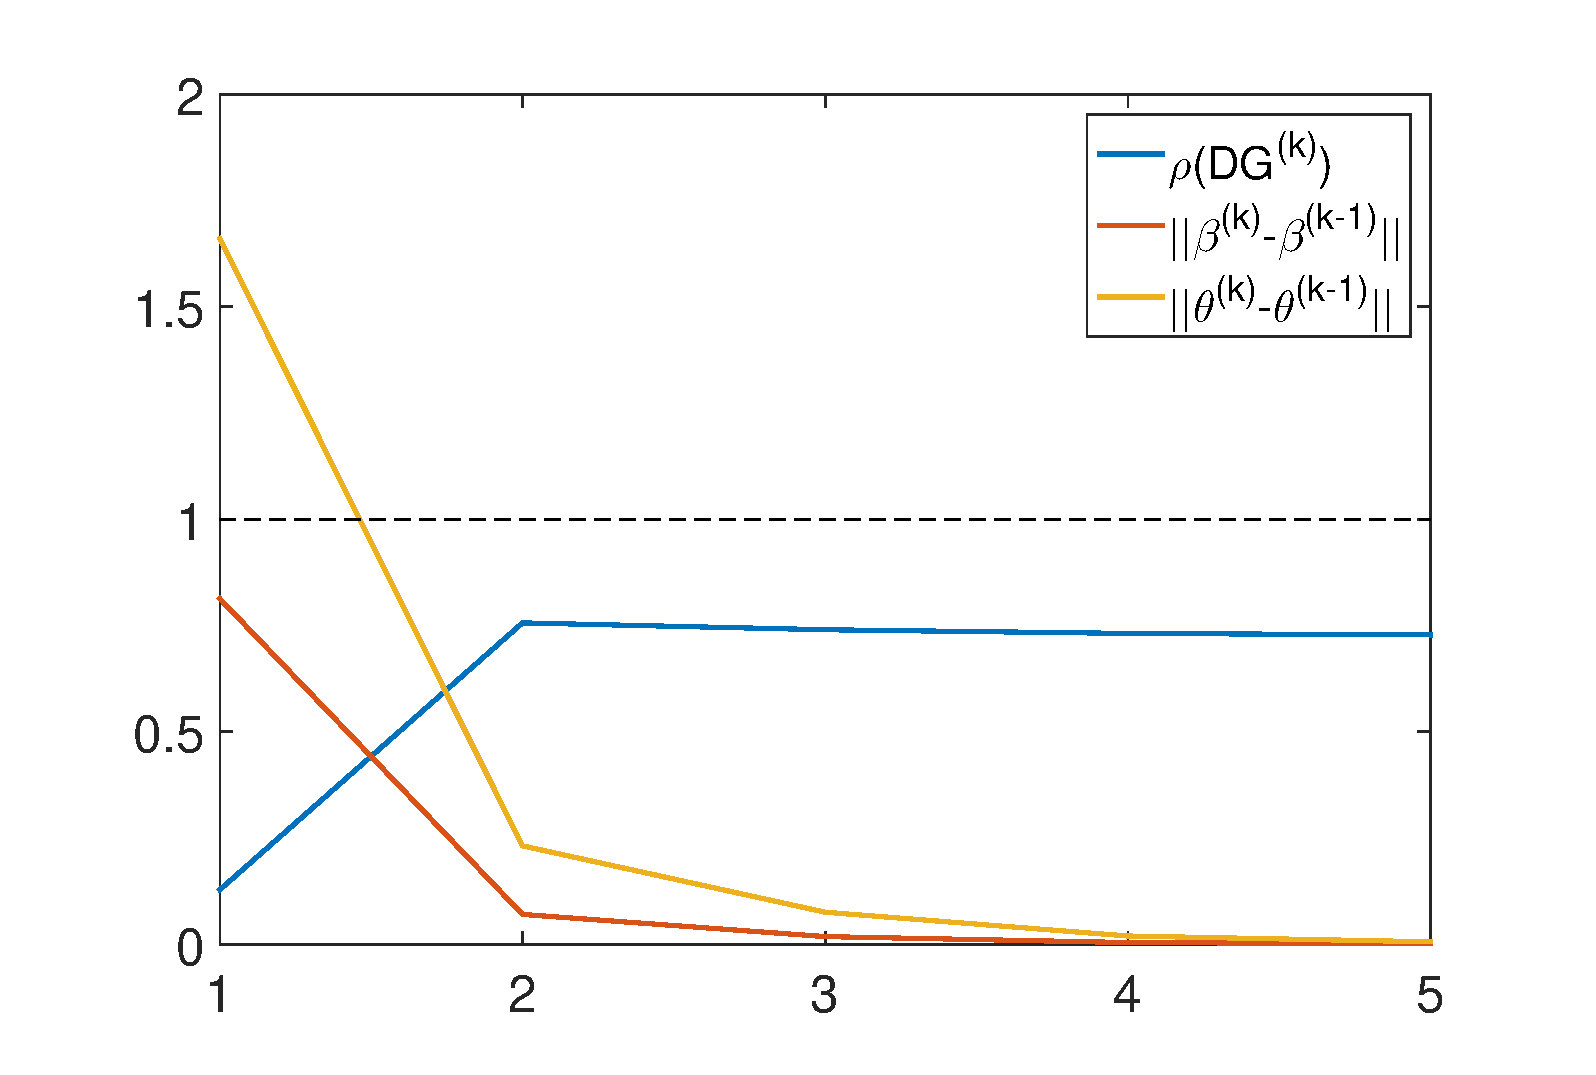
\includegraphics[scale=0.3]{diagnosticsNKPC.eps} }
       \subfigure[Iterative E-stability of the unique $\boldsymbol \beta^{*}$]{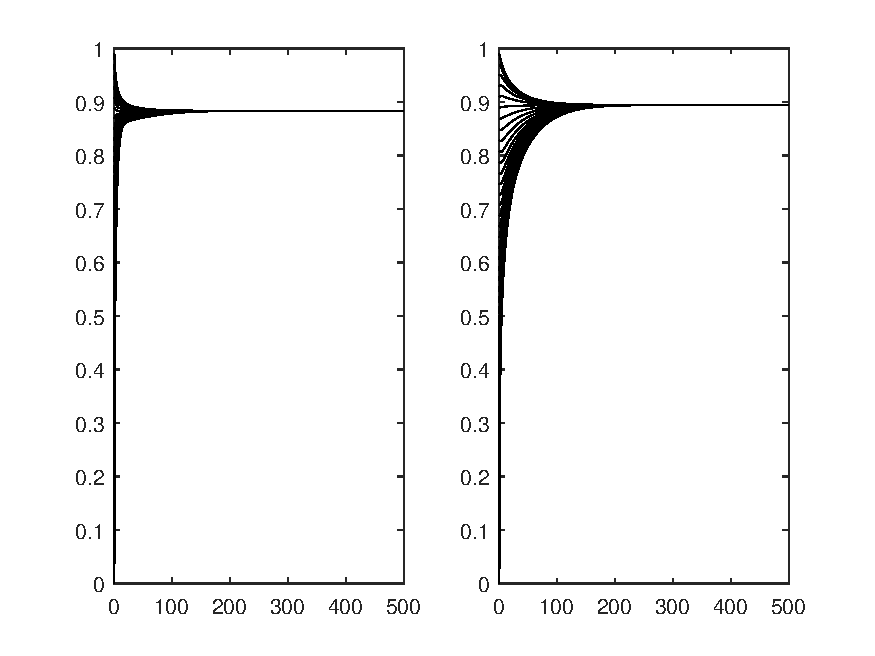
\includegraphics[scale=0.5]{NKPC_estimated_fixedPoint_iter.pdf}}}\\
 
      \caption{The estimated BLE is $(\beta_y^*,\beta_{\pi}^*)=(0.88, 0.89)$. The left panel shows the largest eigenvalue, and the norm distances between consecutive values of $\pmb{\beta^{(k)}}$, as well as $\theta^{(k)}$ across iterations. The second panel shows convergence towards the unique (iteratively) E-stable BLE with randomized initial values.}     
      \label{nkm_convergence}
\end{figure}
    

    \begin{figure}
    \mbox{\subfigure[$\beta_y^{*}$ and $\beta_{\pi}^{*}$ under constant gain learning.]{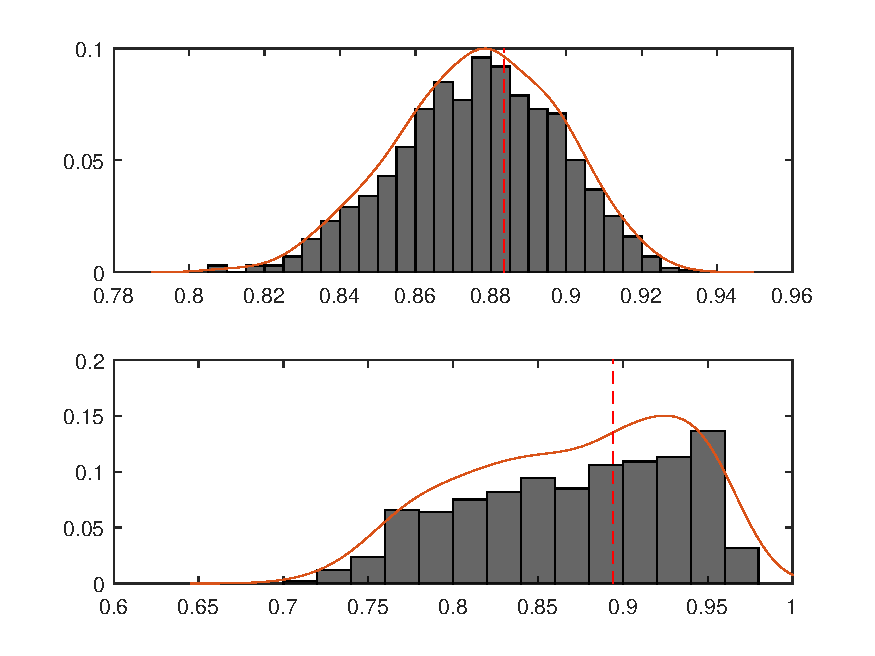
\includegraphics[scale=0.55]{NKPC_MC_cgl.pdf}}
 \subfigure[$\beta_y^{*}$ and $\beta_{\pi}^{*}$ under decreasing gain learning.]{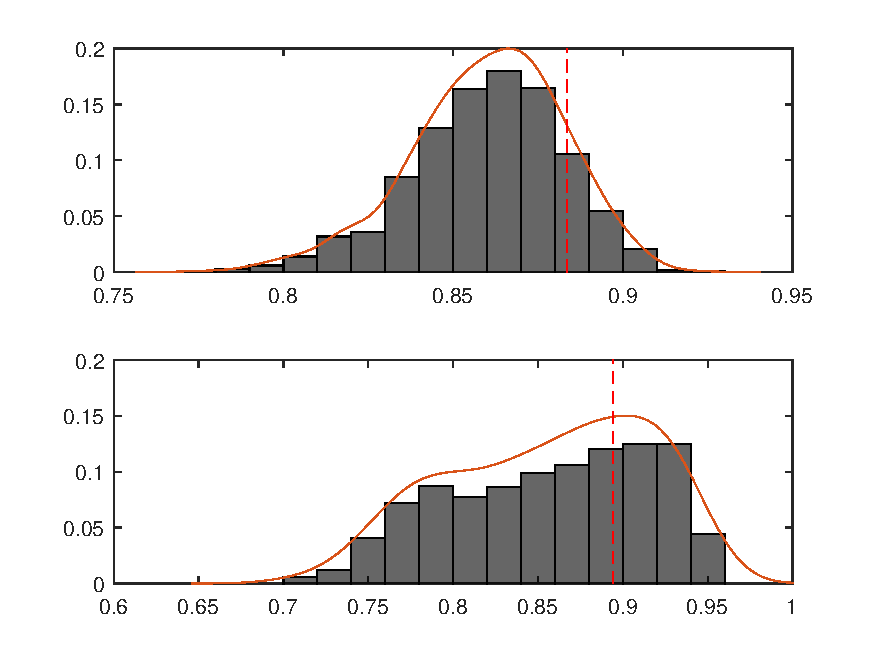
\includegraphics[scale=0.55]{NKPC_MC_dgl.pdf}}}\\

  \caption{ Monte Carlo Simulations: frequency distributions and unimodality test for $\beta_y$ and $\beta_{\pi}$ resulting from 1000 simulations. Hartigan's unimodality test p-values are $ 0.98$ and $0.94$ for $\beta_y$ and $\beta_{\pi}$  under constant gain simulations, and $ 0.99$ and $0.99$ for the decreasing gain simulations. Hence the null hypothesis of unimodality is not rejected for any of the distributions.
   }
  \label{nkm_sac_MC}
\end{figure}

\begin{figure}
    \centering

    \vspace{3 mm}
    \mbox{\subfigure[Filtered Variables and mean parameters]{
    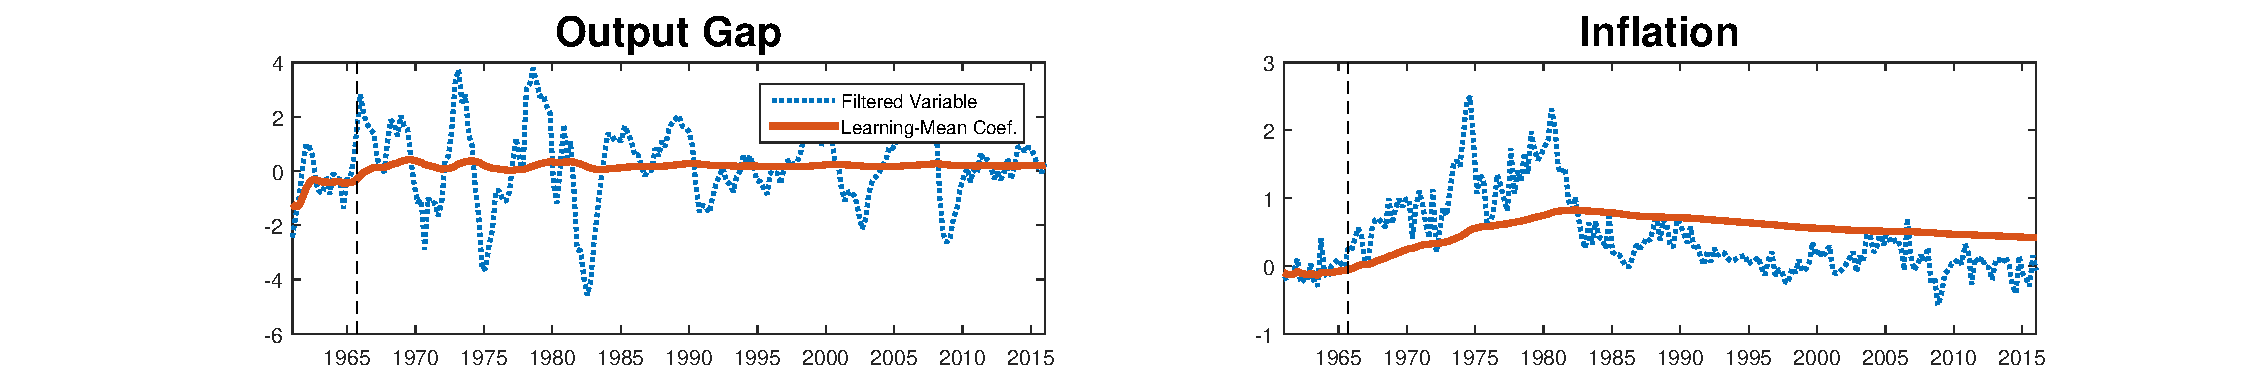
\includegraphics[scale=0.5]{NKPC_alphas.pdf}}}\\
     \mbox{\subfigure[Persistence parameters]{
    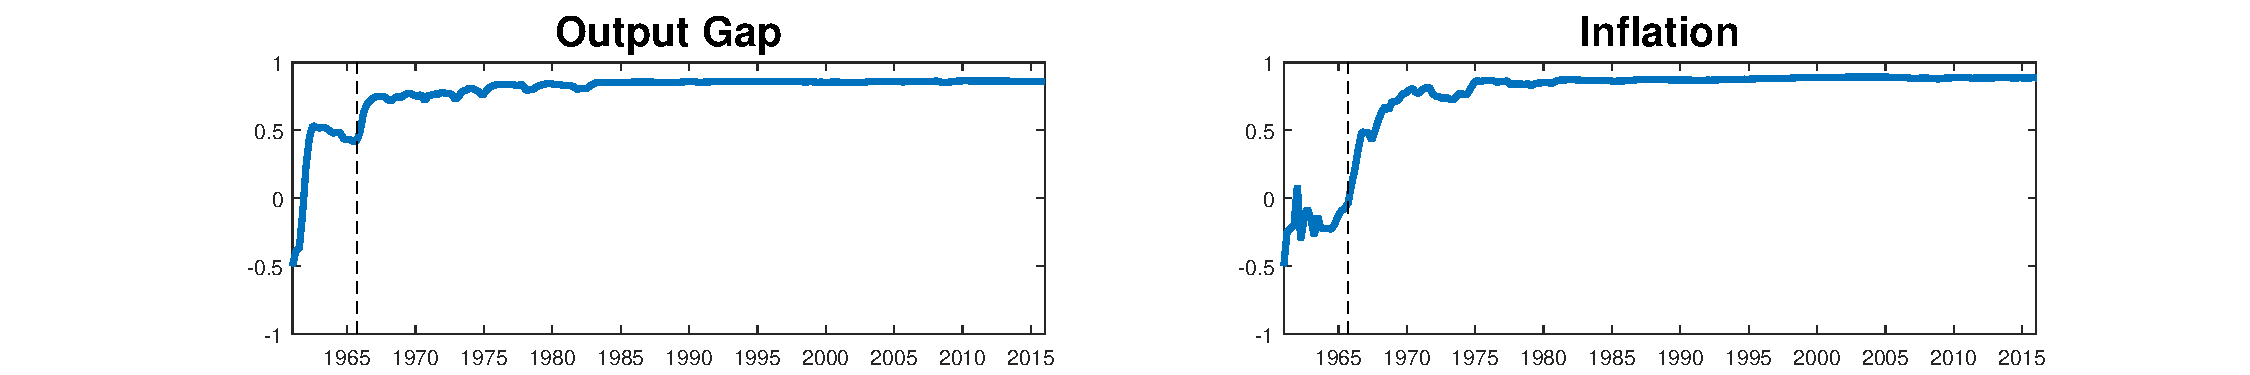
\includegraphics[scale=0.5]{NKPC_betas.pdf}}}\\
    
        \caption{Filtered variables and learning parameters over the estimation sample under SAC-learning, where Kalman filter output is used to update the belief coefficients. Converged values of first-order autocorrelations are $0.86$ and $0.89$ for output gap and inflation respectively.}
    \label{nkpc-sac-figure}
\end{figure}

Overall, our results suggest important differences in the estimated parameters and the propagation of shocks under BLE. These changes lead to a substantial improvement in the empirical fit, evident from the (log marginal) likelihood of $-337$ under BLE compared with $-348$ under REE, which yields a Bayes' Factor $4.78$ in favour of BLE\footnote{Based on Jeffrey's Guidelines (Greenberg, 2012), if the Bayes' Factor is in favour of a model is larger than 2, then this provides \textit{decisive support} for the model under consideration.}. Comparing the results to SAC-learning, it is readily seen that there are no substantial differences with the BLE specification. Relative to the REE estimations, the exogenous shocks have lower persistence and larger standard deviations, the risk aversion coefficient is lower, Phillips curve slope is higher and monetary policy coefficients are similar. The only difference with the BLE model arises in the steady-state values of inflation and interest-rate, which turn out lower under the SAC-learning estimation. This difference arises since the learning coefficients are time-varying under real-time SAC-learning and Figure \ref{nkpc-sac-figure} suggests that they are slightly above zero on average, which drives down the estimates of the steady-state parameters\footnote{Shutting off the learning dynamics about mean coefficients and letting the agents learn only about the first-order autocorrelations indeed yields steady-state values similar to BLE.}. Other than these small differences, all parameter estimates are fairly close under BLE and SAC-learning, with implied HPD-intervals well within the range of each other. The likelihood turns out to be $-341$ under SAC-learning, which is still better than the fit of REE, with a Bayes' Factor of 3.08 in favour of SAC-learning, but worse than BLE, with a Bayes' Factor of 1.7 in favour of BLE\footnote{Based on Jeffrey's Guidelines, this provides \textit{very strong} evidence in favour of BLE.}. This result suggests that transitory dynamics and the resulting time-variation in the learning parameters do not improve the model fit in our decreasing-gain learning setup. Overall, these results also allow us to illustrate the advantage of using Algorithm II to estimate a BLE: the estimation under SAC-learning requires a relatively large burn-in sample for the convergence of first-order autocorrelation coefficients. This might become an issue if the researcher does not have a sufficiently long dataset, as is typical in most quarterly macroeconomic time series. Furthermore, as we have already seen in Figure \ref{nkm_sac_MC}, the simulations under learning have a relatively large Monte-Carlo variance. In other words, while the simulations converge to the underlying BLE on average, there might be relatively large deviations from the underlying fixed-point for any given simulation. Hence what comes out of the estimation in a real-time learning setup is similar to a single simulation of the model under learning, which in general may not accurately reflect the underlying fixed-point. In the following, we check whether these results are robust to different measures of output gap and different subsamples for the BLE and REE specifications.


%\subsection{Impulse Responses}






%\begin{figure}

%\textbf{One standard deviation shocks (at the estimated value) on inflation and output. Left panel is BLE, right panel is REE. The grey areas depich the 90 \% confidence bands.}\\

%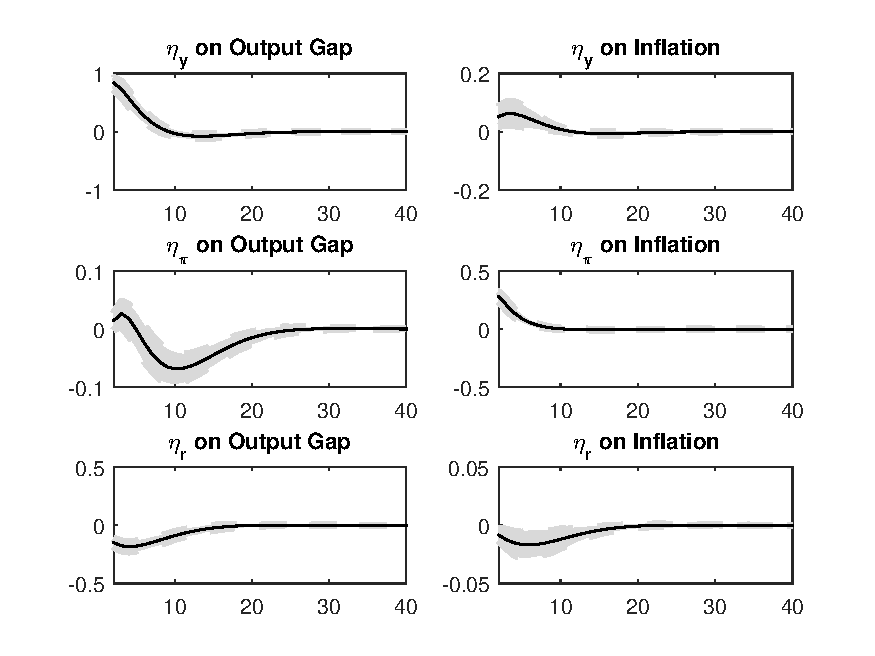
\includegraphics[scale=0.6]{nkpc_ble_irfs.pdf}
%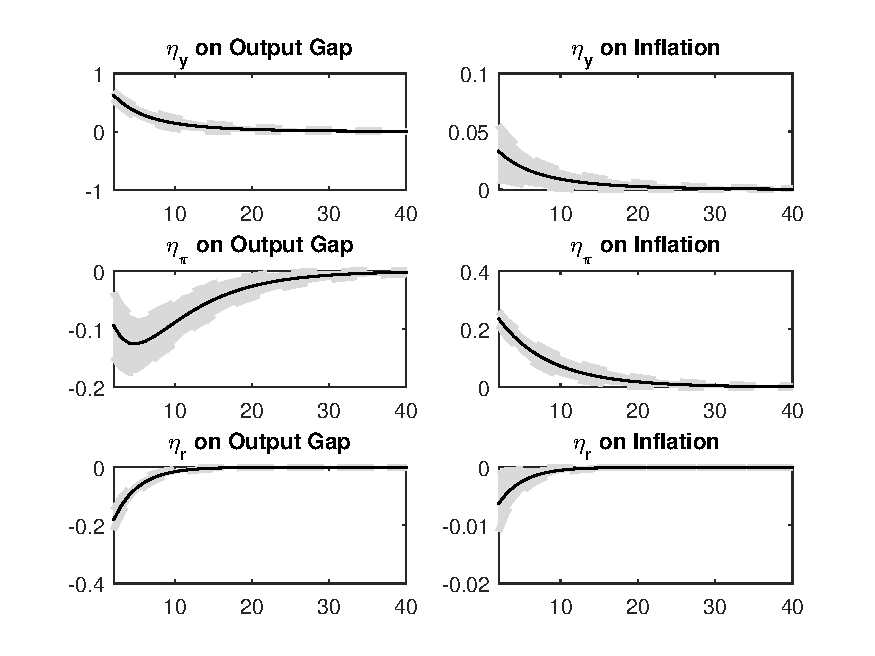
\includegraphics[scale=0.6]{NKPC_ree_irfs.pdf}\\

%\textbf{Comparison of responses under BLE and REE, the shocks are scaled to one under both specifications. }
%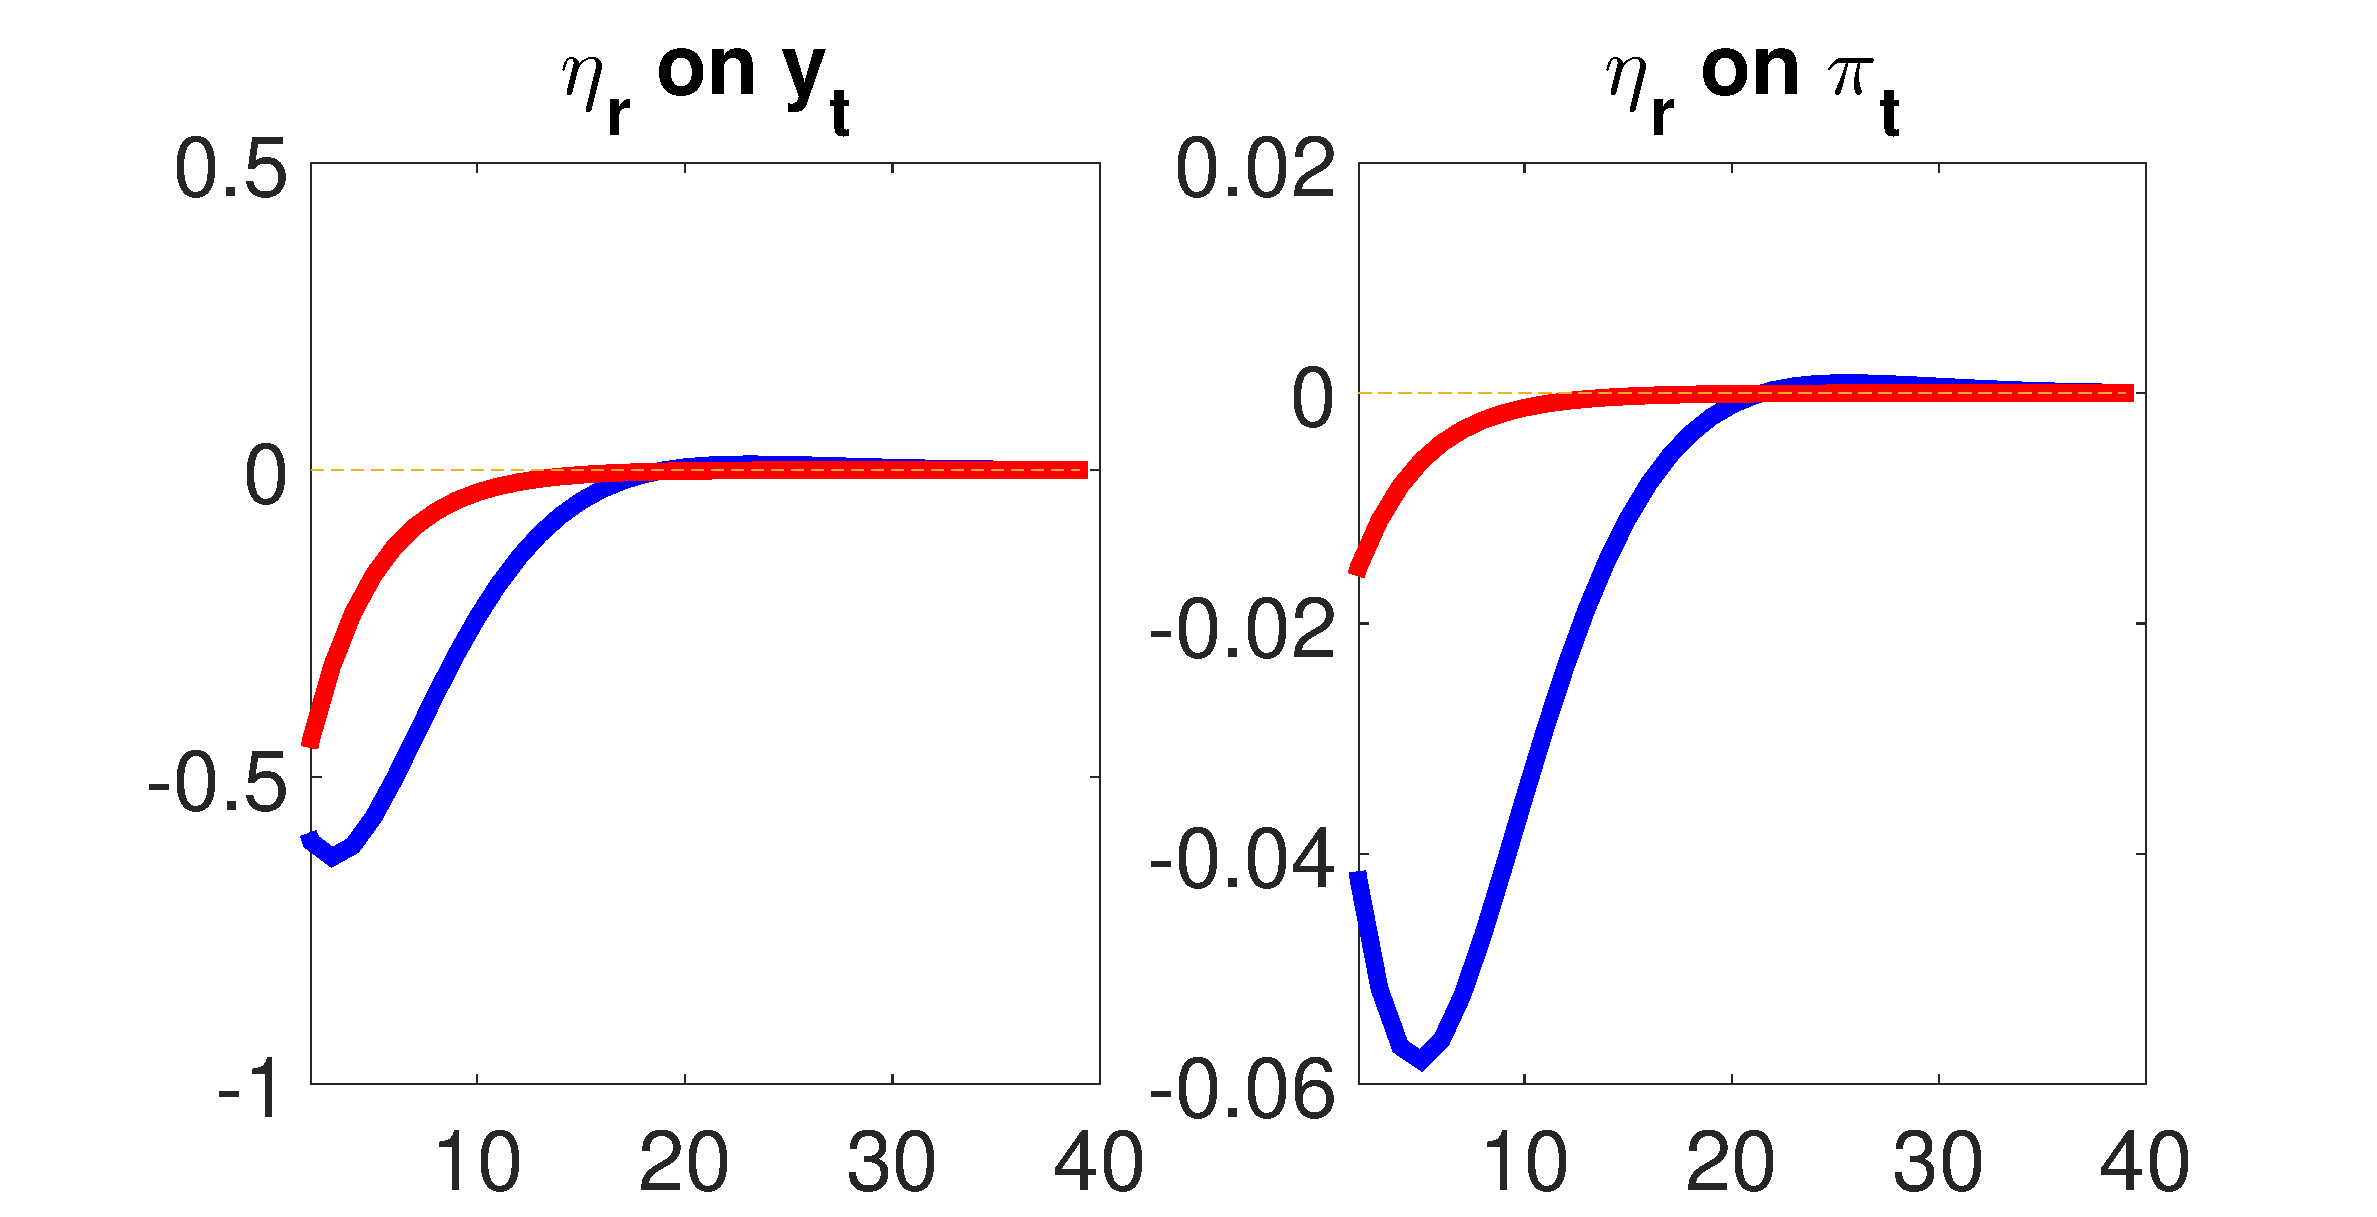
\includegraphics[]{nkpc_irfs_comparison.pdf}
%\end{figure}




\subsubsection*{Subsample Estimations}

We first chek whether our main results hold across different sample periods. To this end, we consider three periods: 1966:I-1979:II, the period before Great Moderation; 1966:I-2008:IV, the period before Great Recession and the zero lower bound episode; and 1984:I-2008:IV, the Great Moderation period. 

\noindent

Table \ref{nkm_subsample} reports the posterior mode and the corresponding Laplace approximation for all periods under BLE and REE. It is readily seen that the difference between parameter estimates are preserved across all three periods: BLE is characterized by lower persistence but larger standard deviation estimates in shocks, a steeper Phillips curve characterized by larger $\gamma$, and a smaller risk aversion coefficient. The estimation under BLE provides a better model fit under all three subsamples, with Bayes' Factors of $1.67$, $3.93$ and $2.44$ in favor of the BLE model. 




\begin{table}[!htbp]
\begin{tabular}{l||ll||ll||ll}
Period & 66:I-79:II &  & 66:I-08:IV & & 84:I-08:IV \\
\hline
\hline
 & BLE & REE & BLE & REE & BLE & REE\\
Laplace & -118.63 & -122.47 & -313.16 & -322.10 & -34.32 & -39.93 \\
\hline
Bayes Factor & 1.67 &  & 3.93 &  & 2.44 & \\
\hline
\hline
Parameter & Mode &  &Mode  &   & Mode \\
\hline
\hline
$\eta_y$ &    0.94 & 0.24 &     0.76 & 0.17 &   0.53 & 0.09\\
$\eta_{\pi}$ & 0.38 & 0.06 & 0.3 & 0.04 &       0.18 & 0.08\\
$\eta_r$     & 0.20 & 0.20 & 0.31 & 0.32 &      0.15 & 0.15\\
$\bar{y}$ & -0.22 & -0.14 &   -0.09 & -0.14 &    0.05 & -0.14\\
$\bar{\pi}$ & 0.93 & 0.75 &     0.84 & 0.71 &   0.61 & 0.58 \\
$\bar{r}$ & 1.03 & 0.86 &    1.25 & 1.08 &      1.14 & 0.97\\
$\gamma$ & 0.054 & 0.01 &     0.033 & 0.006 &   0.046 & 0.007\\
$\frac{1}{\psi}$ & 2.44 &   2.77 & 4.03 & 3.78 & 2.82 & 3.15\\
$\phi_{\pi}$ & 1.03 & 1.07 & 1.29 & 1.31 &      1.55 & 1.57\\
$\phi_y$ & 0.39 & 0.36 &     0.45 & 0.42 &      0.48 & 0.54\\
$\rho_y$ & 0.5 & 0.87 &     0.42 & 0.88 &       0.44 & 0.94\\
$\rho_{\pi}$ & 0.31 & 0.85 & 0.32 & 0.87 &      0.24 & 0.55\\
$\rho_r$ & 0.72 & 0.68 &     0.83 & 0.77 &      0.9 & 0.85\\
\end{tabular}
\caption{Comparison of the sub-sample estimations under BLE and REE.}
\label{nkm_subsample}
\end{table} 
%\afterpage{\clearpage}


\subsubsection*{Alternative Definitions of Output Gap}

Next we check whether our results are sensitive to which measure of output gap is considered by using two alternative definitions: output gap based on de-trended output, 
%\footnote{De-trending here is based on a $4^{th}$ order polynomial, which yields the best fit over our main sample.} 
and output gap based on CBO's measure of potential output. The estimations over our main sample are reported in Table \ref{nkm_alt_gap}, which yield the same conclusions as before:  BLE is characterized by lower persistence but larger standard deviation estimates in shocks, a steeper Phillips curve characterized by larger $\gamma$, and a smaller risk aversion coefficient. The likelihood is also better under BLE for both definitions, with Bayes' Factors of $11.49$ and $10.41$ respectively. As a final check, we compare the likelihoods across the three sub-samples with the alternative measures of output gap, which is reported in Table \ref{nkm_alt_subs}: it is readily seen that the likelihood under BLE is better for both measures under all sub-samples, although the difference for the Great Moderation period 1985-I:2008:IV is much smaller. These results are also consistent with our previous findings. \\




\begin{table}[!htbp]
\centering


\begin{tabular}{l||ll||ll}
 &     BLE det. &   REE det.   & BLE CBO.   & REE CBO.\\
 Laplace&      -360.96   & -387.42   & -342.9  & -366.88 \\
 \hline
 Bayes Factor &       11.49   &    & 10.41  &  \\
\hline
\hline
&        Post.  &  & Post. & \\
\hline
 Parameter & Mode &   Mode & Mode & Mode\\
$\eta_y$   &      0.78 &   0.08 &   0.74   & 0.11\\
$\eta_{\pi}$ &  0.3 &   0.04 &   0.29 &   0.04 \\
$\eta_r$ &     0.3   & 0.31   & 0.29   & 0.3 \\
$\bar{y}$  &     -0.13 &   -0.19   & -0.54 &   -0.42\\
$\bar{\pi}$    &  0.79 &   0.66 &   0.81 &   0.59 \\
$\bar{r}$ &      1.09 &   0.92 &   1.15 &   1.05 \\
$\gamma$  &     0.017 &  0.004 &   0.024 &   0.006\\
$\frac{1}{\psi}$  &       2.92 &   4.86   & 2.65 &   4.57 \\
$\phi_{\pi}$  & 1.44 &   1.45 &   1.41 &   1.43 \\
$\phi_y$  &     0.22 &   0.16 &   0.36 &   0.27 \\
$\rho_y$ &      0.42 &   0.88 &   0.42 &   0.89 \\
$\rho_{\pi}$  &  0.31 &   0.94 &   0.31 &   0.92 \\
$\rho_r$ &      0.88 &   0.79 &   0.88 &   0.8 
\end{tabular}
\caption{Alternative estimations of the 3-equation NKPC model: we compare the results under BLE and REE with two alternative specifications of output gap. In the first case output gap is defined as the deviation of output from a quadratic trend, while in the latter we take the output gap based on CBO's measure of potential output.  }
\label{nkm_alt_gap}
\end{table}

\begin{table}[!htbp]
\centering

\begin{tabular}{l||ll||ll||ll}
& 66:I-79:II & & 66:I-08:IV  & & 84:I-08:IV & \\
\hline
\hline

& BLE & REE & BLE & REE & BLE & REE  \\
\hline
\hline

CBO's estimate & -126.07 & -127.6 & -321.9 & -344.4 & -36.7 & -46.9\\
\hline
Bayes Factor & 0.66 &   & 9.77 &   & 4.43 &  \\
\hline
\hline
Detrended output & -129.9 & -133.1 & -333.1 & -353.2 & -48.4 & -66.9\\
\hline
Bayes Factor & 1.39 &   & 8.73 &   & 8.03 &  \\
\end{tabular}
\caption{Sub-sample estimations with alternative definitions of output gap. } 
\label{nkm_alt_subs}
\end{table}
%\afterpage{\clearpage}


\FloatBarrier
